%!TEX root = ../../../memoria.tex
\section{\checkoutEF}\label{chapter:solucionimplementada:section:checkout}

	Mientras sea posible, hay que limitar el proceso de \checkoutEF a una sola página. En el caso de separar el proceso en algunas páginas, se debe incluir una barra de proceso para mostrar cuanto falta para terminar \cite{online_official_imediaconnection_best_practices_shopping_cart}
	% Try to keep it to one page
	% If at all possible, limit the checkout process to a single page. If you must spread it out across a few pages, include a progress bar to show people how far they have left to go.
	% Read more at http://www.imediaconnection.com/content/36794.asp#6qlTEqOcCeTePmFQ.99

% TODO obserar esto para conectar bien 
	El proceso consiste en 6 pasos que deben cumplirse para que se cree la orden.

	En la parte superior de esta vista( \refFigura{figure:checkout:global_status}), se puede ver en todo momento el estado actual del \workflowCPT del proceso \checkoutEF.

	\begin{figure}[H]
		\centering
		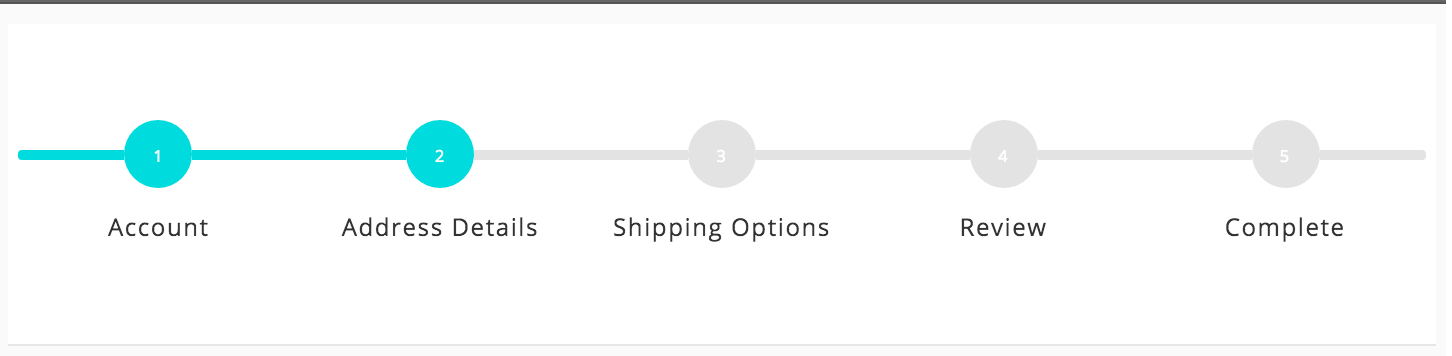
\includegraphics[width=0.7\textwidth]{figuras/shipping/global_status.png}
		\caption{Estado actual del \workflowCPT del \shippingEF. En este caso se encuentra en la selección de la dirección.}
		\label{figure:checkout:global_status}
	\end{figure}

	Adicionalmente a eso, la vista de \shippingEF muestra en detalle todos los pasos (\refFigura{figure:checkout:steps}). Cada uno de estos pasos se define como:

	\begin{description}
		\item[Account] \hfill \\
			Corresponde al proceso de autenticarse en la plataforma.
		\item[Address Details] \hfill \\
			Paso para la selección de una de las direcciones configuradas. Si no se tiene ningúna dirección agregada, el sistema muestra inmediatamente el formulario para la creación de una nueva dirección (\refFigura{figure:checkout:form_address}).
		\item[Shipping Options] \hfill \\
			Permite seleccionar uno de los métodos de envío disponibles. Estos son configurados por el administrador 
		\item[Review] \hfill \\
			Muestra un resumen de la información agregada al carro de compra. 
		\item[Complete] \hfill \\
			Paso de selección de método de pago.
	\end{description}


	\begin{figure}[H]
		\centering
		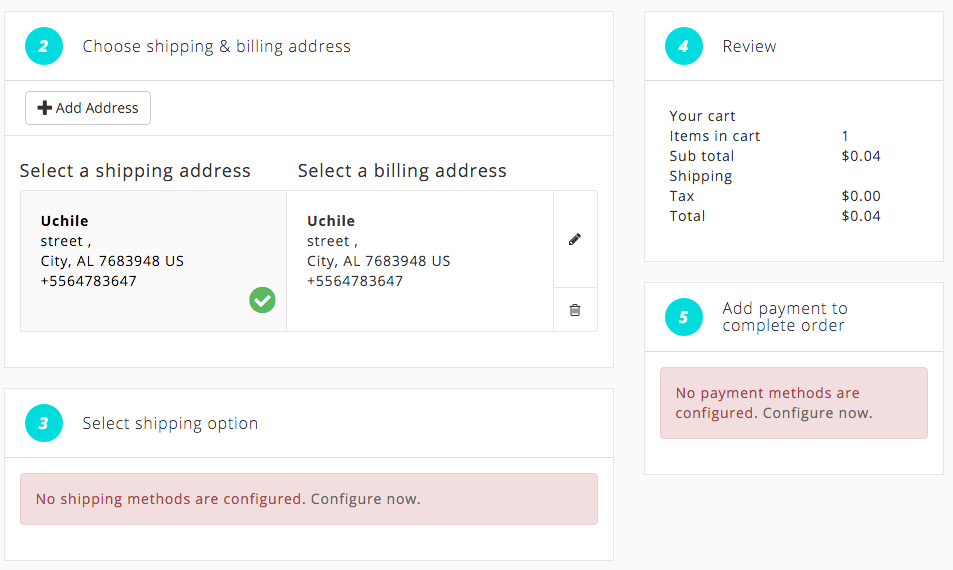
\includegraphics[width=0.8\textwidth]{figuras/shipping/steps.png}
		\caption{Detalle de todos los pasos del \workflowCPT \shippingEF.}
		\label{figure:checkout:steps}
	\end{figure}

	%TODO: modificar este texto despues
	En la \refFigura{figure:checkout:steps} se observa que los pasos 3 y 5 tienen un mensaje advirtiendo que no hay métodos de \shippingEF y métodos de pago configurados. Esta configuración debe ser realizada por el o los administradores de la tienda. Pero actualmente no están disponibles las interfaces para realizar estas acciones.

	\begin{figure}[H]
		\centering
		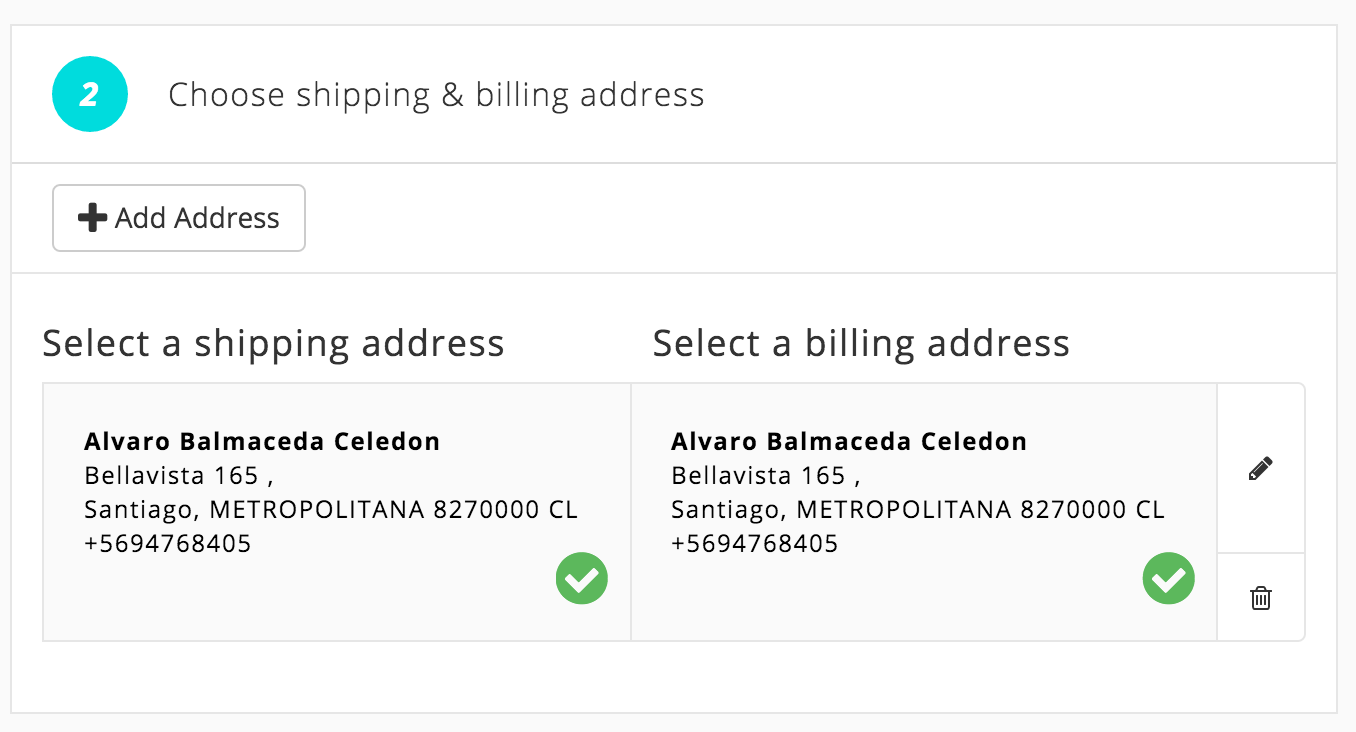
\includegraphics[width=0.8\textwidth]{figuras/shipping/step_address.png}
		\caption{Seleccionar dirección en proceso de \shippingEF.}
		\label{figure:checkout:step_address}
	\end{figure}

	\begin{figure}[H]
		\centering
		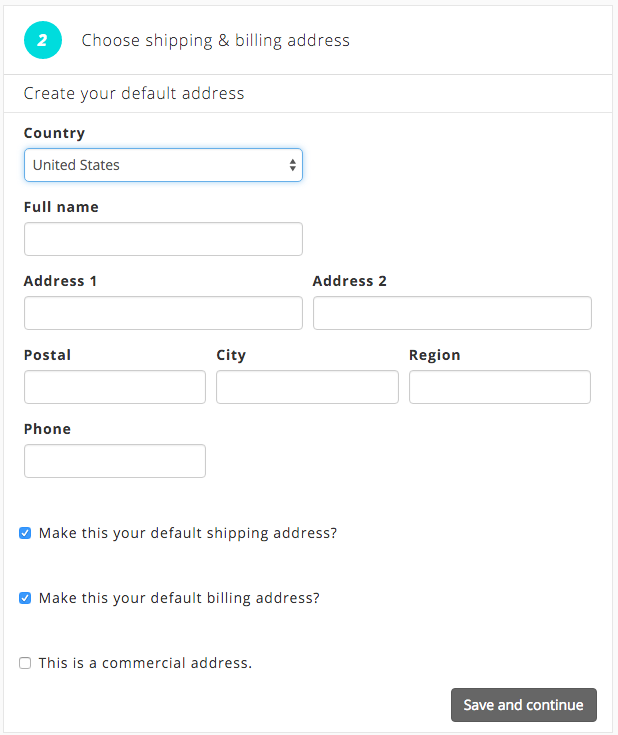
\includegraphics[width=0.6\textwidth]{figuras/shipping/form_address.png}
		\caption{Despliegue automático del formulario de direcciones cuando no se tienen ninguna dirección agregada.}
		\label{figure:checkout:form_address}
	\end{figure}


	En el caso de tener direcciones configuradas, pero se desee hacer el envío a una nuseva dirección, es posible crearla apretando el botón \textit{Add Address} y un formulario se desplegará (\refFigura{figure:checkout:form_add_address}). Este formulario es equivalente al de la \refFigura{figure:checkout:form_address}, pero este incluye la opción de cancelar la creación de la dirección.

	\begin{figure}[H]
		\centering
		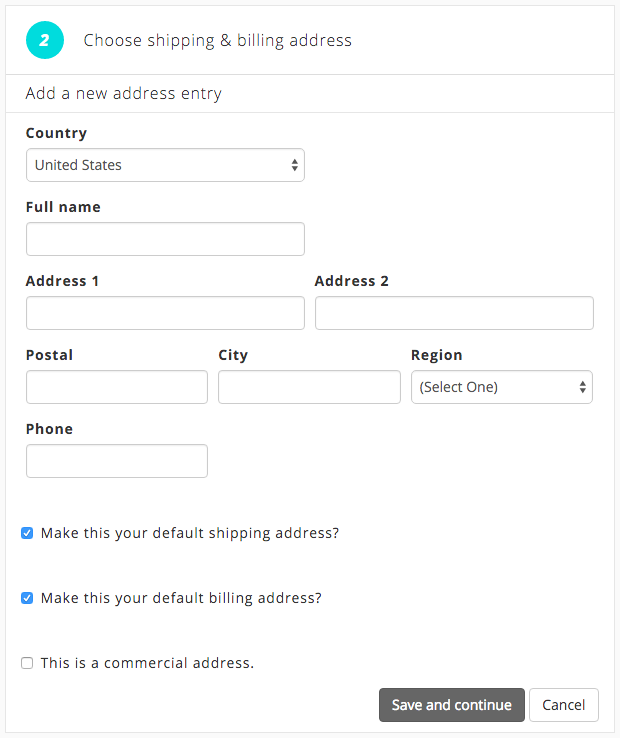
\includegraphics[width=0.6\textwidth]{figuras/shipping/form_add_address.png}
		\caption{Formulario de creación de una nueva dirección. Se diferencia del formulario de la \refFigura{figure:checkout:form_address} en que este incluye el botón Cancel.}
		\label{figure:checkout:form_add_address}
	\end{figure}




	% caracteristicas actuales en cuentas de usuarios
	%!TEX root = ../../../../memoria.tex
\subsection{\paymentsCOM}\label{chapter:solucionimplementada:section:payment}
	
	Como se mencionó en la sección \ref{cap:solucionImplementada:section:dashboard:subsection:payment} \nameref{cap:solucionImplementada:section:dashboard:subsection:payment}, es relevante considerar varios métodos de pagos, sin embargo en el contexto de esta memoria solo se ha integrado a \PPPaymentProNAME.


	\subsubsection{\PPPaymentProNAME}
		Anteriormente se había indicado que este método permite mantener a los clientes dentro del \websiteINT durante el proceso completo de \paymentsCOM y \checkoutCOM. Básicamente se ha implementado la aceptación de pago de tarjetas de crédito a través de un formulario dentro del \websiteINT. La información necesaria para la transacción se ve en \refCodigo{source:javascript:checkout:payment:paypal_accept_payments}.

		% JSON con la información necesaria para aceptar el pago con tarjetas de crédito
		%!TEX root = ../../../../memoria.tex

\medskip
\begin{lstlisting}[caption= Estructura de un \itemcollection, label=source:javascript:checkout:payment:paypal_accept_payments]
{	
	"intent": "sale",
	"payer":{
		"payment_method": "credit_card",
		"funding_instruments": [
			{
				"credit_card": {
					"number": "5500005555555559",
					"type": "mastercard",
					"expire_month": 12,
					"expire_year": 2018,
					"cvv2": 111,
					"first_name": "Betsy",
					"last_name": "Buyer"
				}
			}
		]
	},
	"transactions": [
		{
			"amount": {
				"total": "7.47",
				"currency": "USD"
			},
			"description": "This is the payment transaction description."
		}
	]
}
\end{lstlisting}

		De acá se desprende la información de la tarjeta:

		\begin{itemize}
			\item Número.
			\item Tipo de Tarjeta.
			\item Mes en que expira la tarjeta.
			\item Año en que expira la tarjeta.
			\item \cvvTWOCOM.
			\item Nombre.
			\item Apellido.
		\end{itemize} 

		Toda esta información debe ser entregada por el cliente, con el fin de gestionar el pago. Sin embargo, se sabe que el tipo de tajeta puede ser determinado a partir de los 6 primeros dígitos del número de tarjeta \cite{online_investopedia_meaning_IIN}. 

		Los campos de expiración de tarjeta de crédito pueden ser confusos para decifrar si no son escritos exactamente como están en las tarjetas de crédito. Algunos \websitesINT usan nombres de meses, mientras otros emplean una combinación de \nombreNumeroCPT, mientras y usan solo números. La manera correcta de dar los campos de formato es simplemente poner los campos de la misma manera en que aparecen en la tarjeta de crédito (solamente números). Esto minimiza la confusión y mala interpretación porque el usuario puede fácilmente verificar  los campos contra los de la tarjeta de crédito \cite{online_official_smashingmagazine_fundamental_guidelines_checkout_design}.

		Finalmente, se desarrolla el formulario de la \refFigura{figure:checkout:payment:paypal_payflow:form}, para que el cliente pueda efectuar el pago del producto y/o servicio.

		\begin{figure}[H]
			\centering
			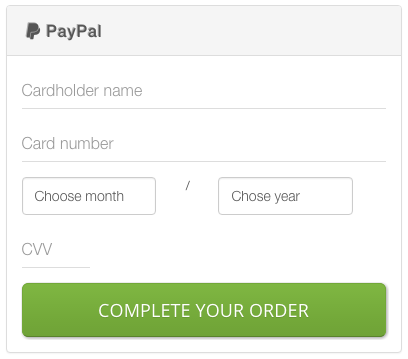
\includegraphics[width=0.6\textwidth]{figuras/payment/credit_card_form.png}
			\caption{Formulario de la tarjeta de crédito para realizar el pago utilizando \PPPaymentProNAME.}
			\label{figure:checkout:payment:paypal_payflow:form}
		\end{figure}

		%TODO: agregar referencia a la interfaz de orde de compra.
		Una vez finalizado este proceso, se creará una orden de compra, la cual podría ser consultado en la interfaz de ordenes.